\chapter{Research background}
	\label{chap:background}
	
\section{Deep Learning}

\section{General information on adversarial examples}

\subsection{Generating adversarial examples}

Generating adversarial perturbations in white-box setting is an optimisation problem, and there is a wide variety of formulations of the problem in the literature. Szegedy \textit{et al.} \cite{szegedy2014intriguing} first defined it in the targeted setting as finding the minimum perturbation $\delta$ such that the victim model $f$ computes the desired wrong label $y^\prime$:

\begin{equation}
\label{eq:szegedy_1}
\begin{aligned}
\min_{\delta} \quad & c\|\delta\|_2\\
\textrm{s.t.} \quad & f(x + \delta) = y^\prime\\
  &x + \delta \in [0,1]^m \textrm{, m is the number of pixels in image}   \\
\end{aligned}
\end{equation}

Because equation \ref{eq:szegedy_1} is a very hard optimisation problem, Szegedy \textit{et al.} \cite{szegedy2014intriguing} use a relaxed form of the problem, where the constraint regarding the desired output is included in the objective function:

\begin{equation}
\label{eq:szegedy_2}
\begin{aligned}
\min_{\delta} \quad & c\|\delta\|_2 + L(f(x + \delta), y^\prime)\\
\textrm{s.t.} \quad& x + \delta \in [0,1]^m \textrm{, m is the number of pixels in image}   \\
\end{aligned}
\end{equation}

In equation \ref{eq:szegedy_2}, $L$ represents the loss function of the victim model. We want to minimise the loss in regards to the desired wrong label to increase the chance that the victim model will produce that output when the adversarial input is given.

Another paper \cite{silva_survey} defines the problem for untargeted adversarial attacks as:

\begin{equation}
\begin{aligned}
\max_{\delta} \quad & L(f(x + \delta), y)\\
\textrm{s.t.} \quad& \|\delta\|_2\leq\epsilon   \\
\end{aligned}
\end{equation}

Here, maximising the loss in regards to the true label increases the chance that the model will not give that output. For targeted attacks, they define it as :

\begin{equation}
\label{eq:silva}
\begin{aligned}
\max_{\delta} \quad & L(f(x + \delta), y) - L(f(x + \delta), y^\prime)\\
\textrm{s.t.} \quad& \|\delta\|_2\leq\epsilon   \\
\end{aligned}
\end{equation}

In equation \ref{eq:silva}, the second term ensures that the loss function in regards to the desired wrong label is minimised.

In most papers on the subject, the optimisation problem constrains the size of the perturbation vector $\delta$ \cite{akhtar, silva_survey, tnnls_survey}. It does so by making sure that the perturbation vector's $\ell_2$ or $\ell_\infty$ norm is smaller than the maximum threshold $\epsilon$. This is to ensure that the perturbation is not too noticeable to the human eye. $\epsilon$ is often called \textbf{perturbation budget} in the literature. The $\ell_0$ norm is used by some attacks \cite{akhtar} which only want to change as few pixels as possible. 

The optimisation problem is usually solved through gradient descent. Szegedy \textit{et al.} \cite{szegedy2014intriguing} used a box constrained L-BFGS optimiser. Goodfellow \textit{et al.} \cite{fgsm} developed FGSM, a fast one-step attack method that is very popular in the literature. It calculates the gradient of the loss function of the target classifier at the given input and multiplies its sign with a constant scalar to obtain a perturbation that will change the output label.  Basic Iterative Method is an iterative version of FGSM \cite{kurakin2016adversarial} and is equivalent to the L$\infty$ version of Projected Gradient Descent \cite{madry2019deep}, which is itself a popular method to create adversarial examples. On the other hand, generative networks can also be used instead of gradient descent to create adversarial perturbations \cite{upset_angri, zheng_black_box_GAN, advGAN}. These methods will be presented in more detail in subsection \ref{sec:generative_models}. 

Akhtar and Mian \cite{akhtar} provide a very useful table summarising many attack methods and whether they are white-box or black-box, targeted or untargeted, and what perturbation vector norm they use.

\subsection{Taxonomy of adversarial attacks}

Akhtar \textit{et al.} \cite{akhtar} wrote the first comprehensive literature review on adversarial attacks and defences in deep learning for computer vision. The authors show a comprehensive list of attacks, but do not provide a useful taxonomy and only classify them based on the architecture type of the targeted neural network. 

On the other hand, a later survey \cite{silva_survey} categorises attacks based on several criteria. Depending on the \textbf{information} the attacker knows, an attack may be \textbf{white-box} or \textbf{black-box}. In the former, the attacker has full access to the architecture and parameters of the victim model, while in the latter the attacker does not have this knowledge. Dong \textit{et al.} \cite{dong2020benchmarking} further divides black-box attacks into three categories: transferability-based attacks, score-based attacks, where the attacker can query the victim model for soft-label predictions on chosen input, and then estimate the gradient, and decision-based attacks, where the attacker can only query for hard-label predictions, for which it is harder to estimate the gradient.

Attacks can also be classified depending on the \textbf{goals} of the attacker. \textbf{Untargeted} attacks only seek to make the victim model output a wrong result, whatever it may be. Meanwhile, \textbf{targeted} attacks have the goal of making the victim compute a specific wrong label. Furthermore, most attacks produce \textbf{image-specific} perturbations, which are designed to work for one specific image only. However, Moosavi-Dezfooli \textit{et al.} \cite{Moosavi-Dezfooli_2017_CVPR} discovered a method of creating \textbf{universal} adversarial noise, which induces misclassification when applied to the vast majority of images in the dataset. Finally, attacks can be categorised based on the \textbf{attack frequency}, whether the adversarial noise is generated in one step, such as in FGSM \cite{fgsm}, or in an iterative process, like in \cite{carlini2017towards}.

\subsection{Applicability of adversarial attacks}
  
Ever since the publication of \cite{szegedy2014intriguing}, most of the research has been on CNNs for object recognition tasks \cite{akhtar}. However, adversarial attacks are possible on other architectures, such as GANs \cite{kos_attacks_on_gans}, autoencoders \cite{tabacof_attacks_autoencoders}, recurrent neural networks \cite{papernot_attacks_rnns} and neural networks for semantic segmentation of an image \cite{Metzen_2017_ICCV}. Moreover, autoencoders are much more resilient against adversarial attacks \cite{tabacof_attacks_autoencoders}, and the experiments done by Tang \textit{et al.} \cite{robustart} show that Vision Transformers are more robust against adversarial attacks than CNNs.

\subsection{Transferability}

Transferability-based black-box attacks succeed due to a property of adversarial examples, first discovered in \cite{szegedy2014intriguing}, that they often manage to fool victim models that are different than the model for which the adversarial example was originally made. This can happen even if the two models have different architectures. Therefore, an attacker can create adversarial perturbations for a substitute model that they control and then use them to mount an attack against another model with inaccessible parameters and loss function gradient. Dong \textit{et al.} \cite{mim} use an optimisation method with momentum to create transferability-based attacks. Meanwhile, ANGRI \cite{upset_angri} is a generative model which learns to create adversarial perturbations by using 3-4 substitute models. Similarly, Zheng \textit{et al.} \cite{zheng_black_box_GAN} train their generator against a substitute model, and they analyse four different substitute models. Their experiments show that CNNs which use depth-wise separable convolution \cite{xception} produce stronger adversarial perturbations when used as simulators.

\subsection{Why do adversarial examples exist?}

While Silva and Najafirad \cite{silva_survey} do not cover why adversarial examples exist, Akhtar and Mian \cite{akhtar} report that there are varied and sometimes contradictory viewpoints in regards to this problem and that there is no consensus. However, they claim that the hypothesis in Goodfellow \textit{et al.} \cite{fgsm} is the most popular. This hypothesis says adversarial attacks are caused by the fact that most neural networks are too linear, which is supported by the existence of the FGSM \cite{fgsm} attack method. This excessive linearity could be caused by the popular ReLU activation function, which is piece-wise linear. In Krotov and Hopfield \cite{krotov2018dam}, experiments show that neural networks with highly non-linear activation functions can not be fooled by adversarial examples generated by models equivalent to DNNs with ReLU activation, therefore supporting the linearity hypothesis. 

On the other hand, Tanay and Griffin \cite{tanay2016boundary} contradict this and show that some linear image classifiers are not vulnerable to adversarial attacks. They hypothesize that adversarial examples exist because naturally occurring data samples exist on a subspace of the total input space and that adversarial examples exist when the classification boundary lies too close to this sub-manifold. Therefore, small perturbations manage to move the input across the decision boundary. On the other hand, their experiments show that if the decision boundary is perpendicular to this sub-manifold, the model is more robust against attacks. It is worth noting that their explanation does not totally contradict the linearity hypothesis, as the behaviour they describe is still quite linear.

On a different line of thought, Ilyas \textit{et al.} \cite{adv_examples_bugs} hypothesize that images contain subtle features that are useful for maximising the classification accuracy but are semantically meaningless in regards to the object in the photo. Adversarial perturbations that resemble "non-robust" these features make the victim model misclassify the adversarial examples with very high confidence.

\subsection{Defences against adversarial attacks}

Akhtar and Mian \cite{akhtar} classified defences to adversarial attacks as follows: modified input/training, modifying the neural networks, or adding external models as add-ons. However, their classification is confusing, as they list SafetyNet, which uses an SVM to detect adversarial perturbations besides the DNN, as modifying the network and not as an add-on. Silva and Najafirad \cite{silva_survey} provide another classification: gradient masking, used so that the attacker can not use the loss function gradient to create adversarial examples, adversarial example detection and robust optimisation. The latter includes adversarial training, where adversarial examples labelled with the correct label are added to the training set, certified defences, where the model is proven formally to be resistant against perturbations up to a certain limit, and regularisation. The authors put a lot of emphasis on certified defences and seem to disregard the effectiveness of adversarial training. However, Dong \textit{et al.} \cite{dong2020benchmarking} performed extensive experiments that show that adversarial training often leads to more robust models than other defences based on regularisation or certified defence.

\section{Adversarial attacks in the physical world}
\subsection{Challenges}

Most attacks, including the one in figure \ref{fig:adversarial_segmentation} on page \pageref{fig:adversarial_segmentation}, directly add the perturbations to the whole image. In a realistic setting, the attacker can not directly manipulate the pixels of the input, especially when the model takes its input from sensors. Furthermore, physical adversarial examples, whether 2D printed images or 3D objects, can have their fooling rate diminished by the angle they are viewed from, their distance from the camera, lighting conditions, the inability of the sensor to pick up the subtle adversarial perturbations, and perhaps colour printing errors \cite{kurakin2016adversarial, athalye, evtimov_road_signs}.

Kurakin \textit{et al.} \cite{kurakin2016adversarial} were among the first who investigated adversarial attacks in the physical space. They created adversarial images using FGSM \cite{fgsm}, printed them and took a picture of the printed photos using a smartphone. They then used automatic perspective transformation and cropping to transform the picture, then ran the classifier on it and compared the attack success with the original adversarial example. Over 66.67\% of adversarial examples still fooled the victim model after being printed and photographed. Therefore, it was proven that adversarial examples apply to the physical domain.

However, the photographs taken in \cite{kurakin2016adversarial} only had slight variations in terms of the camera lighting, camera distance and camera angle. Meanwhile, Lu \textit{et al.} \cite{lu_physical_experiments} did similar experiments to the ones in \cite{kurakin2016adversarial}, except they tried a wide variety of camera angles and distances, and they found that the adversarial examples were successful only when the camera was in certain positions. For example, the accuracy of the model doubled or almost tripled when the camera distance increased from 0.5m to 1.5m. Therefore, they concluded that adversarial examples may not be a serious threat to neural networks used in cyberphysical systems.

\subsection{Expectation over Transformation}
    \label{subsubsec:eot}

To rectify the shortcomings of adversarial attacks shown in Lu \textit{et al.} \cite{lu_physical_experiments}, Athalye \textit{et al.} \cite{athalye} proposed the Expectation over Transformation (EOT) framework. It is designed to create adversarial examples that are effective in physical settings, and can work on 3D rendered objects as well as 2D images. Their key innovation is that they model transformations such rotation, translation, perspective projection, 3D rendering or lighting in the optimisation search for the adversarial noise. Therefore, they formulate the following optimisation problem:

\begin{equation}
\begin{aligned}
\max_{x^\prime} \quad & (\mathrm{E}_{t\sim T}[log P(y_{t} | t(x^\prime))] - \lambda \mathrm{E}_{t\sim T}[d(t(x^\prime), t(x))])\\
\textrm{s.t.} \quad & x \in [0, 1]^d   \\
\end{aligned}
\end{equation}

\noindent where t is a function which simulates the various transformations, $x^\prime$ is the adversarial version of x, $\lambda$ is a chosen penalty constant, and d measures the perceptual difference between x and $x^\prime$. 

The first term maximises the log probability that the neural network will classify the adversarial example as the desired target label $y_{t}$. While $x^\prime$ is the input that the attacker directly controls, t(x) is the input seen by the neural network. In the 3D case, x is a 2D texture and t(x) is a 3D rendered object with that texture, seen from a particular angle and distance. You can see an example of this in figure \ref{fig:rendering}. The 3D rendering process is formally considered as a linear transformation such that $t(x) = Mx + b$, which is differentiable.

\begin{figure}[h]
    \centering
    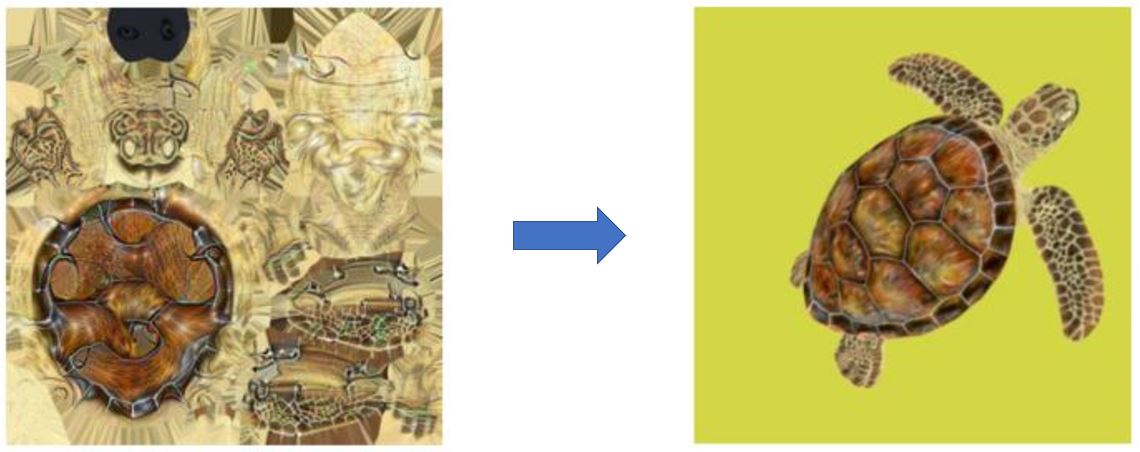
\includegraphics[width=0.8\textwidth]{graphics/rendering.JPG}
    \caption{The transformation function can model the rendering of a 2D texture into a 3D object with a specific pose. Images are taken from \cite{athalye}.}
    \label{fig:rendering}
\end{figure}

Meanwhile, the second term minimises the distance between the adversarial example and the original input. The authors use this formulation instead of $x^\prime - x$ to focus on the effective distance between the two, as the classifier sees t(x) rather than x.

In each optimisation step, the authors use the mean gradient over a mini-batch of 40 images, each being a different transformation of the same original image. 32 of those are re-used from the previous mini-batch, while the other 8 are new images created with 8 new transformation functions drawn from the distribution $T$. By using this process, they ensure that the adversarial object remains adversarial even though it is viewed from a wide variety of perspectives.

This framework leaves three things up to the choice of the attacker: the distribution of transformation functions $T$, the distance metric $d$ and the optimisation algorithm for maximising equation 5. For the latter, the authors used projected gradient descent. In the experiments with 3D rendered and physical objects, according to the supplementary material of \cite{athalye}, the parameters for the camera distance, translation, rotation of the object, lighting and 3D printer colour error are each drawn from an independent uniform distribution.

Meanwhile, the distance metric that they used is:

\begin{equation}
\begin{aligned}
d(t(x^\prime), t(x)) = \|LAB(t(x^\prime)) - LAB(t(x))\|_2
\end{aligned}
\end{equation}

\noindent where $LAB(t(x))$ is the projection in LAB space of the image vector $t(x)$. LAB is a colour space where the Euclidean distance between two colour vectors is roughly equivalent to how different the human eye perceives those colours to be. The authors chose this metric so that the adversarial noise is less obvious to humans.

To test the EOT framework for generating 3D adversarial objects, the authors evaluated 200 adversarial examples with 100 random transformations each, and found that they were classified as the wrong target label 96.4\% of the time, while being classified correctly only 0.9\% of the time. For comparison, the accuracy is 68.8\% on the original 3D objects. Following that, Athalye \textit{et al.} created two 3D-printed adversarial objects, a baseball and a turtle, and found that they were classified as the target label 59\% and 82\% of the time, respectively. You can see some photos of the turtle in figure \ref{fig:3d_turtle}. Consequently, we can conclude that the EOT framework can synthesize physical 3D adversarial objects that remain highly effective when viewed from a variety of view points.

\begin{figure}[h]
    \centering
    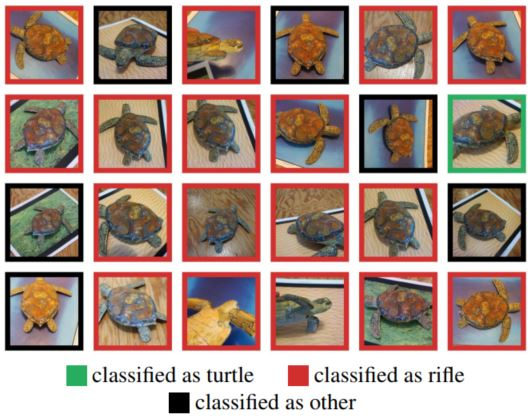
\includegraphics[width=1\textwidth]{graphics/turtle.JPG}
    \caption{A selection of photographs of the 3D adversarial turtle object. The adversarial perturbation was made for the "rifle" target label. Taken from \cite{athalye}.}
    \label{fig:3d_turtle}
\end{figure}

\subsection{Robust Physical Perturbations}

Concurrently to the work presented in subsection \ref{subsubsec:eot}, Eykholt \textit{et al.} \cite{evtimov_road_signs} developed a similar method for creating robust physical-world attacks, called Robust Physical Perturbations ($\textrm{RP}_2$). It is geared towards adversarial perturbations for 2D physical objects, such as traffic signs. 

In contrast with EOT \cite{athalye}, where the transformation functions sample from $T$ synthetically augmented the dataset by placing the rendered 3D object in various poses, here the authors augment the dataset by manually taking photos of the original object from various angles and distances and in varying lighting conditions. They further use some synthetic transformations in the form of cropping and changing the image brightness to add new transformed images to the dataset. The input to $\textrm{RP}_2$ is a photo of an object taken from its front, and during the optimisation process, they draw a new sample from a distribution $X$ of images of that same object, seen under various transformations.

Moreover, because the input to $\textrm{RP}_2$ is an image of the physical 3D object rather than a 2D texture of an object, the authors use a mask $M_x$ to make sure that the adversarial perturbation $\delta$ is only applied to object itself and not to the image background. The mask is a matrix the size of the image, with a 0 for each pixel where no perturbation should be added, and 1 otherwise. 

With these changes in mind, the authors of \cite{evtimov_road_signs} define the optimisation problem in $\textrm{RP}_2$ as:

\begin{equation}
\begin{aligned}
\min_{\delta} \quad & \lambda\|M_x \cdot \delta\|_p + NPS + \mathrm{E}_{x_i\sim X}J(f_\theta(x_i + T_i(M_x \cdot \delta)), y_t)\\
\label{eq:rp2}
\end{aligned}
\end{equation}

\noindent where $NPS$ is a term for correcting printing colour errors, $J(\cdot, \cdot)$ is the loss function of the classifier represented by $f_\theta$, $y_t$ is the adversarial target label and $T_i$ is a function that transforms the perturbation to match the object in the image. If the object is seen from a 30\degree{} angle, the perturbation is rotated by 30\degree{} in 3D. The first term is for minimising perturbation, and the third term ensures that the adversarial example is misclassified.

Eykholt \textit{et al.} used $\textrm{RP}_2$ to create a poster of a driving STOP sign, with perturbations applied to the whole surface of the sign. They manually took photos of the poster from a variety of distance and angles, and 100\% these photos were misclassified as $y_t$ by a CNN, with an average confidence of 80.51\%. In another experiment, they created adversarial patches in the form of a stickers and placed them over a a real STOP sign. Just like in the previous experiment, they took photos of the sign and then fed them into the CNN. The attack with regular stickers had a 100\% success rate, and an attack with a sticker which looked like a graffiti succeeded 66.67\% of the time.

\section{Generative Models}
    \label{sec:generative_models}
    
\subsection{GANs and autoencoders}
    
This subsection will introduce some common generative model architectures that are relevant for this project.

\textbf{Generative Adversarial Networks} (GAN) is a framework first proposed in Goodfellow \textit{et al.} \cite{gans}. It consists of a generator which creates new data samples and a discriminator whose job is to tell which samples are real or generated. The generator is trained to create samples which the discriminator network can not distinguish from real data. The generator and discriminator are each trained alternatively, several steps at a time. GANs have proven to be very powerful and are capable of generating highly realistic photos of people \cite{styleGAN}.

\textbf{Autoencoders} are a type of neural network that is used to learn an appropriate latent representation of data. It is made up of an encoder and a decoder. The encoder reduces the input into a smaller latent vector and it often takes the shape of a neural network without a softmax layer. The decoder takes the latent vector as input and uses deconvolutional layers to generate new data. Auto-encoders are usually trained to reconstruct the original image from the latent space, though they can be used to generate something else too.

\subsection{Generative model for creating black-box attacks}
    \label{subsubsec:zheng}

Zheng \textit{et al.} \cite{zheng_black_box_GAN} proposed a generative model for creating targeted black-box adversarial examples for 2D images. Its architecture consists of two components, a generator and a simulator. The purpose of the simulator is to act as a substitute for the black-box victim model, while the generator creates adversarial noise for a given image and target label.

The simulator is trained so that it provides the same output as the victim model for a given adversarial example created by the generator:

\begin{equation}
\begin{aligned}
\min_{\theta_s} \quad & L(S(\theta_s, x + G(x, z)),V(\theta_v, x + G(x, z)))\\
\textrm{s.t.} \quad & x \in X, \|G(x, z)\|_\infty < \delta
\label{eq:simulator_loss}
\end{aligned}
\end{equation}

\noindent where the outputs predicted by the simulator and victim model are denoted by $S(\cdot,\cdot)$ and $V(\cdot,\cdot)$, respectively. $\theta_s$ and $\theta_v$ are the parameters of the simulator and victim model, respectively. The adversarial noise created by the generator for a given image $x$ and a given target label $z$ is written as $G(x,z)$. $X$ is the training set and $\delta$ is the perturbation budget. Equation \ref{eq:simulator_loss} is visualised in figure \ref{fig:simulator_loss}.

\begin{figure}[h]
    \centering
    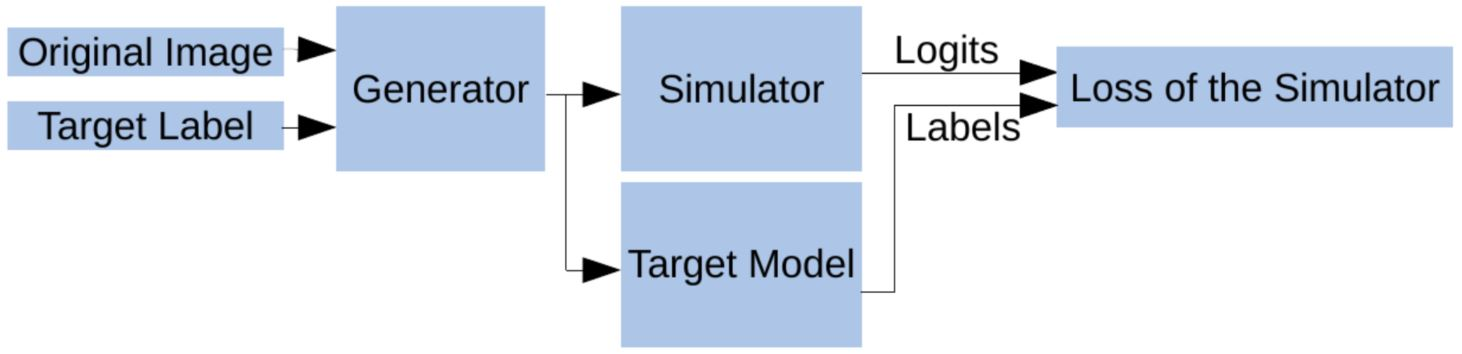
\includegraphics[width=1\textwidth]{graphics/simulator_loss.JPG}
    \caption{Computational flow of the loss function for training the simulator. Diagram taken from \cite{zheng_black_box_GAN}.}
    \label{fig:simulator_loss}
\end{figure}

Meanwhile, the generator is trained to fool the simulator such that the latter will classify the generated adversarial noise with the desired wrong label $z$. Training the generator takes the following form:

\begin{equation}
\begin{aligned}
\min_{\theta_g} \quad & L(S(\theta_s, x + G(x, z)),z) + \beta\|G(x,z)\|_2\\
\textrm{s.t.} \quad & x \in X, z \in Y \setminus \{y\}\\
\label{eq:generator_loss}
\end{aligned}
\end{equation}

\noindent where $\theta_g$ is the parameter vector of the generator, $Y$ is the set of labels and $y$ is the correct label of $x$. $\beta$ is a constant for the perturbation size penalty. Figure \ref{fig:generator_loss} visualises the generator training process.

\begin{figure}[h]
    \centering
    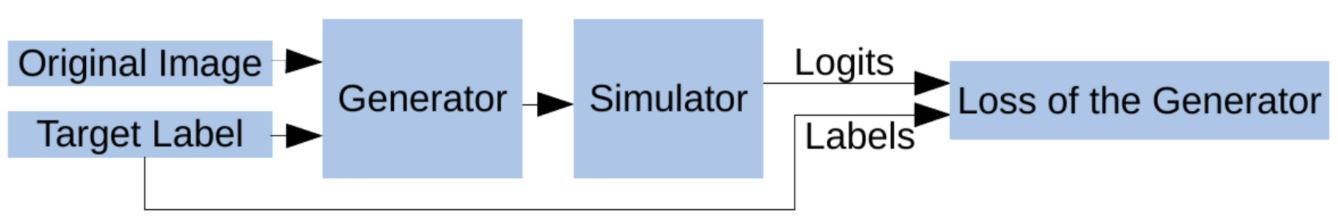
\includegraphics[width=1\textwidth]{graphics/generator_loss.JPG}
    \caption{Computational flow of the loss function for training the generator. Diagram taken from \cite{zheng_black_box_GAN}.}
    \label{fig:generator_loss}
\end{figure}

Because the authors perform adversarial attacks for object recognition, they use various CNNs as simulators, including the Xception model \cite{xception}. Moreover, the proposed generator is an auto-encoder, as you can see in figure \ref{fig:generator}. The encoder takes the form of a CNN without fully connected layers or a softmax layer, and its job is to encode an image as a smaller vector in latent space. The decoder is an ensemble of neural networks made out of deconvolutional layers, and its output is the adversarial perturbation. 

\begin{figure}[h]
    \centering
    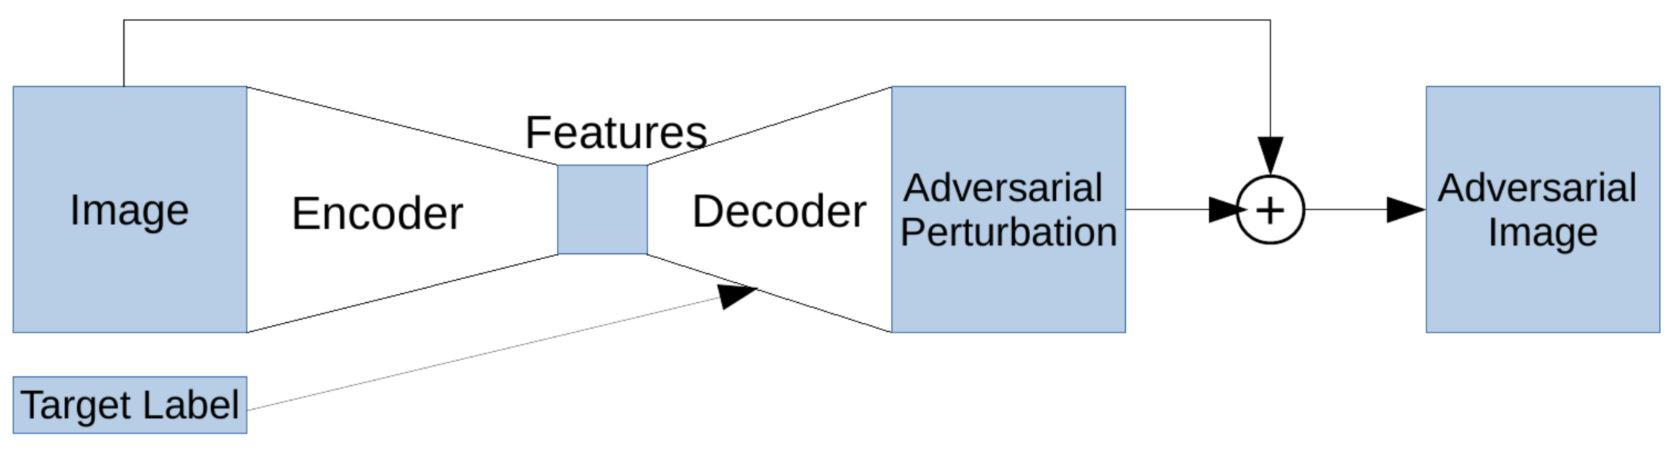
\includegraphics[width=1\textwidth]{graphics/generator.JPG}
    \caption{The autoencoder architecture of the generator in \cite{zheng_black_box_GAN}. Diagram taken from \cite{zheng_black_box_GAN}.}
    \label{fig:generator}
\end{figure}

The decoder uses an ensemble of expert models because the perturbation must be designed for a given target label. The decoder has a gating sub-network inspired by \cite{experts_mixture_gate} which outputs a sparse weights vector based on the target label. The output of the decoder is a weighted sum of the outputs of each expert model, using the weights from the gating network. The decoder will use different combinations of expert models for different target labels.

The targeted adversarial examples produced by Zheng \textit{et al.} \cite{zheng_black_box_GAN} had an average success rate of over 80\% on the CIFAR-10 dataset and of 68.55\% on CIFAR-100. We can therefore conclude that the generative model described in this subsection is highly effective for black-box adversarial attacks. 

